\documentclass[10pt,twocolumn]{article}

\usepackage[utf8]{inputenc}
\usepackage[T2A]{fontenc}
\usepackage[russian]{babel}

\usepackage{amsmath,amssymb}
\usepackage{graphicx}
\usepackage{geometry}
\usepackage{amsthm}
\usepackage{float}

\newtheorem{proposition}{Предположение}
\newtheorem{remark}{Замечание}

\geometry{
a4paper,
left=2cm,
right=2cm,
top=2cm,
bottom=2cm
}

\title{\textbf{Перевод статьи}}
\author{Петр Н. Вабищевич}
\date{}

\begin{document}

\twocolumn[
\maketitle

\begin{abstract}
    В данной работе мы рассматриваем две неявные схемы для сжимаемых уравнений Эйлера, состоящих из скалярного уравнения адвекции для плотности, векторного уравнения адвекции для скорости и баротропного уравнения состояния. Для пространственной дискретизации используются конечные элементы первого порядка, а интегрирование уравнений по времени осуществляется с помощью схемы обратного Эйлера; однако нелинейность обрабатывается двумя различными способами. Наиболее прямой возможностью является решение нелинейной системы методом Ньютона. Мы показываем, что полученная дискретная полностью нелинейная схема сохраняет массу и импульс. Далее мы применяем двухуровневую схему расщепления по физическим процессам и таким образом расцепляем уравнения сохранения массы и импульса. Полученную схему можно применять итерационно на каждом временном уровне для аппроксимации решения полностью нелинейной схемы. Возможности предложенных схем иллюстрируются численными результатами для двумерной модельной задачи с начальным возмущением плотности. Результаты наглядно демонстрируют, что двух итераций на каждом временном уровне достаточно для получения неосциллирующих результатов без использования каких-либо ограничителей или захвата ударных волн.
    \end{abstract}
\vspace{1.5em}
]

\section{Введение}

Модели механики сплошных сред (см., например, [1,2]) основаны на законах сохранения массы, импульса и энергии. Кроме того, некоторые параметры течения, например плотность, обладают так называемым свойством положительности (монотонности). Хорошо известно, что эти важные свойства дифференциальной задачи механики сплошных сред должны наследоваться их дискретными аналогами [3,4], т.е. вычисленное численное решение должно сохранять массу, импульс и энергию, а если плотность положительна, она должна оставаться положительной на всем временном интервале. Течения идеальных жидкостей описываются уравнениями Эйлера, тогда как уравнения Навье–Стокса применяются к течению вязких жидкостей. Математические аспекты обоснования таких моделей рассматриваются, например, в книгах [5,6]. При обсуждении существования решений в различных пространствах Соболева особое внимание следует уделять принципиальным проблемам положительности (неотрицательности) плотности жидкости. Как уже упоминалось выше (см., например, [7]), это свойство должно наследоваться полностью дискретным аналогом математической модели.

В вычислительной гидродинамике (CFD) наиболее важные проблемы связаны с двумя противоречивыми требованиями. А именно, с одной стороны, необходимо строить монотонные аппроксимации адвективных членов, а с другой — законы сохранения должны выполняться на дискретном уровне. Построению монотонных аппроксимаций посвящено много работ (см., например, [8–10]). В [11,12] рассматриваются стандартные линейные аппроксимации для некоторых основных задач механики сплошных сред (задачи конвекции-диффузии). Классическим подходом к обеспечению монотонности вычисляемых решений гиперболических и конвективно-доминируемых задач является введение искусственной вязкости. Что касается современных методов искусственной вязкости, мы отсылаем читателя к, например, [13–16].

Для дискретизации по пространству консервативные аппроксимации строятся на основе так называемых консервативных (дивергентных) формулировок уравнений механики сплошных сред. Этот подход очень естественно используется в интегро-интерполяционном методе (методе баланса) для регулярных и нерегулярных сеток [17], а также в методе конечных объемов [18,19]. Такие консервативные аппроксимации могут также основываться на методе конечных элементов [20,21], который широко используется в вычислительной гидродинамике [22,23].

Большинство дискретизаций по времени законов сохранения используют явные схемы, которые имеют ограничения устойчивости на шаг по времени. Более того, в таких схемах аналогичные ограничения на шаг по времени обычно накладываются для обеспечения монотонности приближенного решения. Поэтому естественно попытаться применить неявные схемы. Для решения краевых задач для уравнений в частных производных широко используются двухслойные схемы [9,24,25] (\(\theta\)-метод, схемы с весами). Устойчивость двухслойных схем в случае линейных задач, основанная на общей теории устойчивости (корректности) операторно-разностных схем, представлена в [17,26]. В частности, можно сформулировать точные (совпадающие необходимые и достаточные) условия устойчивости, которые формулируются как операторные неравенства в конечномерных гильбертовых пространствах.

Современный уровень исследований характеризуется широким использованием явных схем в вычислительной гидродинамике. Аппроксимации по пространству связаны с высокой точностью решения в гладких областях вместе с адекватным представлением ударных волн и других разрывов. В частности, широко используются метод MUSCL годоновского типа, схема Колгана–ван Лера [27,28]. Основные достижения связаны с построением различных вариантов нелинейных аппроксимаций конвективного переноса. Этот подход наиболее ярко представлен в различных модификациях TVD-схем [29,30]. В настоящее время наибольший интерес представляют взвешенные существенно неосциллирующие схемы (WENO) [31]. Мы сосредоточимся на использовании неявных схем для моделирования сжимаемых течений [32,33]. Вычислительная реализация неявных схем намного сложнее, но при этом мы можем получить безусловную устойчивость и улучшенные свойства монотонности приближенного решения.

В настоящей работе в разделе 2 рассматривается начально-краевая задача для уравнений Эйлера, описывающая течения баротропной жидкости, которые представляют собой законы сохранения массы, импульса и полной механической энергии. Дискретизация по пространству выполняется (см. раздел 3) стандартными элементами Лагранжа для плотности и декартовых компонент скорости. Для вычисления приближенного решения на новом временном уровне используется полностью неявная схема (схема обратного Эйлера первого порядка). Полученное приближенное решение сохраняет массу, а дискретная полная механическая энергия удовлетворяет диссипативной оценке. Полностью неявная схема неудобна для численной реализации и требует больших вычислительных затрат, поскольку она требует решения системы связанных нелинейных уравнений для плотности и скорости. В разделе 4 мы предлагаем схему расщепления, которая относится к классу линеаризованных схем расщепления по физическим процессам [34,35]. Линеаризация проводится по полю адвективного переноса таким образом, что на каждом временном уровне необходимо решать отдельные задачи для плотности и скорости. Эта полностью расщепленная линейная схема может использоваться итерационно для аппроксимации решения полностью нелинейной неявной схемы. Возможности предложенных схем демонстрируются на модельной двумерной задаче с локально возмущенной начальной плотностью и нулевой начальной скоростью (см. раздел 5). Пожалуй, наиболее поразительной особенностью итерационной схемы расщепления является то, что она требует лишь небольшого числа итераций (двух или трех) для получения устойчивых и неосциллирующих результатов. Численно исследуется влияние размера сетки по пространству и времени. Наблюдается, что увеличение шага по времени приводит к монотонизации численного решения. Основным результатом работы является доказательство робастности линеаризованной схемы расщепления. Схема включает раздельное решение стандартных задач адвекции для плотности и скорости и демонстрирует быструю сходимость итераций. Такой подход может быть применен к другим задачам механики жидкости, например, для численного решения начально-краевых задач для сжимаемых уравнений Навье–Стокса. Результаты работы обобщены в разделе 6.


\section{Математическая модель}

В этом разделе мы рассматриваем начально-краевую задачу для уравнений Эйлера сжимаемой жидкости с баротропным уравнением состояния. Система уравнений включает скалярное уравнение адвекции для плотности и векторное уравнение адвекции для скорости с заданной баротропной зависимостью давления от плотности. Ниже обсуждаются законы сохранения массы, импульса и полной механической энергии. В нашем исследовании мы предполагаем, что решение является достаточно гладким. В этом случае течение сжимаемой жидкости описывается соответствующими законами сохранения \cite{6,36}.

\subsection{Баротропная жидкость}

Уравнение неразрывности в ограниченной области \(\Omega\) имеет вид
\begin{equation}
\frac{\partial\rho}{\partial t} +\operatorname{div}(\rho \mathbf{u}) = 0,\quad \mathbf{x}\in \Omega ,\quad 0< t\leq T, \tag{1}
\end{equation}
где \(\rho (\mathbf{x},t) > 0\) — плотность, а \(\mathbf{u}(\mathbf{x},t)\) — скорость. Уравнение импульса может быть записано в консервативной форме
\begin{equation}
\frac{\partial}{\partial t} (\rho \mathbf{u}) + \operatorname{div}(\rho \mathbf{u}\otimes \mathbf{u}) + \operatorname{grad}p = 0,\quad \mathbf{x}\in \Omega ,\quad 0< t\leq T, \tag{2}
\end{equation}
где \(p(\mathbf{x},t)\) — давление. Предполагается, что рассматриваемая жидкость является баротропной, т.е. существует известная зависимость давления от плотности \(p = p(\rho)\) с условием \(\frac{dp}{d\rho} >0\).

Предположим, что границы области являются жесткими, и поэтому на них накладывается условие непроницаемости:
\begin{equation}
(\mathbf{u}\cdot \mathbf{n}) = 0,\quad \mathbf{x}\in \partial \Omega . \tag{3}
\end{equation}
Нам также необходимо задать начальные условия для плотности и скорости:
\begin{equation}
\rho (\mathbf{x},0) = \rho^0 (\mathbf{x}),\quad \mathbf{u}(\mathbf{x},0) = \mathbf{u}^0 (\mathbf{x}),\quad \mathbf{x}\in \Omega . \tag{4}
\end{equation}
Начально-краевая задача (1)--(4) описывает нестационарные течения идеальной баротропной жидкости.

Непосредственное интегрирование уравнения неразрывности (1) по области \(\Omega\) с учетом граничного условия (3) приводит к закону сохранения массы
\begin{equation}
m(t) = m(0),\quad m(t) = \int_{\Omega}\rho (\mathbf{x},t)\,d\mathbf{x}. \tag{5}
\end{equation}

В гильбертовом пространстве \(L_{2}(\Omega)\) определим скалярное произведение и норму стандартным образом:
\[
(\mathbf{w},\mathbf{u}) = \int_{\Omega}\mathbf{w}(\mathbf{x})\mathbf{u}(\mathbf{x})\,d\mathbf{x},\quad \| \mathbf{w}\| = (\mathbf{w},\mathbf{w})^{1 / 2}.
\]
Аналогично определяется пространство вектор-функций \(L_{2}(\Omega)\). Если плотность неотрицательна, закон сохранения массы может быть записан как
\[
\| \rho^{1 / 2}\| = \| \rho_{0}^{1 / 2}\|.
\]
Это соотношение можно рассматривать как априорную оценку для \(\rho^{1/2}\) в \(L_{2}(\Omega)\).

Уравнение (2) непосредственно выражает закон сохранения импульса. Интегрируя это уравнение по \(\Omega\), получаем
\[
\int_{\Omega}\frac{\partial}{\partial t} (\rho \mathbf{u})\,d\mathbf{x} + \int_{\partial \Omega}p(\rho)\mathbf{n}\,d\mathbf{x} = 0.
\]
Таким образом, мы имеем
\begin{equation}
\mathbf {I}(t) = \mathbf {I}(0) - \int_{\partial \Omega}p(\rho)\mathbf {n}\,d\mathbf {x},\quad \mathbf {I}(t) = \int_{\Omega}\rho \mathbf {u}\,d\mathbf {x}. \tag{6}
\end{equation}

Умножая на \(\mathbf{u}\) и принимая во внимание уравнение (1), мы можем переписать уравнение (2) как
\[
\frac{1}{2}\frac{\partial}{\partial t} (\rho |\mathbf{u}|^{2}) + \frac{1}{2}\operatorname{div}(\rho |\mathbf{u}|^{2}\mathbf{u}) + \operatorname{div}(p(\rho)\mathbf{u}) - p\operatorname{div}\mathbf{u} = 0.
\]
Интегрирование по области \(\Omega\) с учетом (3) приводит к
\begin{equation}
\frac{1}{2}\frac{d}{dt}\int_{\Omega}\rho |\mathbf{u}|^{2}\,d\mathbf{x} - \int_{\Omega}p(\rho)\operatorname{div}\mathbf{u}\,d\mathbf{x} = 0. \tag{7}
\end{equation}
Второй член в (7) выражается из ренормализованного уравнения неразрывности. Определим потенциальную функцию давления \(\Pi (\rho)\) из уравнения
\begin{equation}
\rho \frac{d\Pi}{d\rho} -\Pi (\rho) = p(\rho). \tag{8}
\end{equation}
В частности, для идеального газа имеем
\begin{equation}
p(\rho) = a\rho^{\gamma},\quad \Pi (\rho) = a\frac{\rho^{\gamma}}{\gamma - 1},\quad a = \mathrm{const} > 0,\quad \gamma >1. \tag{9}
\end{equation}
Из уравнения неразрывности (1) следует
\begin{equation}
\frac{\partial\Pi}{\partial t} +\operatorname{div}(\Pi \mathbf {u}) + p(\rho)\operatorname{div}\mathbf {u} = 0,\quad 0< t\leq T. \tag{10}
\end{equation}
Интегрирование ренормализованного уравнения неразрывности (10) приводит к выражению
\[
\frac{d}{dt}\int_{\Omega}\Pi\,d\mathbf {x} + \int_{\Omega}p(\rho)\operatorname{div}\mathbf {u}\,d\mathbf {x} = 0.
\]
Добавляя это уравнение к (7), получаем
\begin{equation}
\frac{d}{dt}\int_{\Omega}\left(\frac{1}{2}\rho |\mathbf {u}|^{2} + \Pi (\rho)\right)d\mathbf {x} = 0. \tag{11}
\end{equation}
Таким образом, мы приходим к закону сохранения полной механической энергии:
\begin{equation}
E(t) = E(0),\quad E(t) = \int_{\Omega}\left(\frac{1}{2}\rho |\mathbf {u}|^{2} + \Pi (\rho)\right)d\mathbf {x}. \tag{12}
\end{equation}
Уравнения (5), (6) и (12) представляют собой основные законы сохранения для задачи (1)--(4) при сделанных выше предположениях о гладкости решения.

\subsection{Операторно-дифференциальная формулировка}

Для удобства рассмотрения введем операторы адвективного (конвективного) переноса для системы уравнений Эйлера. Оператор адвекции \(\mathcal{A} = \mathcal{A}(\mathbf {u})\) в дивергентной форме записывается следующим образом:
\begin{equation}
\mathcal{A}(\mathbf {u})\phi = \operatorname{div}(\mathbf {u}\phi). \tag{13}
\end{equation}
Предполагая, что скорость \(\mathbf{u}\) удовлетворяет граничному условию (3), получаем
\begin{equation}
(\mathcal{A}(\mathbf {u})\phi ,1) = 0. \tag{14}
\end{equation}
Уравнение неразрывности (1) может быть записано в форме операторно-дифференциального уравнения:
\begin{equation}
\frac{d\rho}{dt} +\mathcal{A}(\mathbf {u})\rho = 0,\quad 0< t\leq T, \tag{15}
\end{equation}
где использовано обозначение \(\rho (t) = \rho (\mathbf {x},t)\). Аналогично, уравнение (2) записывается в виде
\begin{equation}
\frac{d}{dt} (\rho \mathbf {u}) + \mathcal{A}(\mathbf {u})(\rho \mathbf {u}) + \operatorname{grad}p(\rho) = 0,\quad 0< t\leq T. \tag{16}
\end{equation}
Для системы уравнений (15) и (16) с заданной зависимостью \(p(\rho)\) рассматривается задача Коши, где начальные условия (см. (4)) имеют вид
\begin{equation}
\rho (0) = \rho^{0},\quad \mathbf {u}(0) = \mathbf {u}^{0}. \tag{17}
\end{equation}
Для рассматриваемой задачи (15)--(17) ключевым моментом является свойство (14) оператора адвекции, записанного в дивергентной форме.

\section{Неявная двухслойная схема}

Для численного решения начально-краевой задачи для уравнений Эйлера мы используем полностью неявную схему (обратную схему Эйлера) для шага по времени вместе с дискретизацией по пространству методом конечных элементов. Ниже обсуждается выполнение законов сохранения на дискретном уровне.

\subsection{Дискретизация по пространству}

Для численного решения задачи (15)--(17) мы применяем дискретизации по пространству методом конечных элементов (см., например, [37,38]). Для (13) определим билинейную форму
\[
a(\phi ,\psi) = \int_{\Omega}\operatorname{div}(\mathbf {u}\phi)\psi\,d\mathbf {x}.
\]

Определим подпространство конечных элементов \(V^{h}\subset H^{1}(\Omega)\) и дискретный оператор \(A = A(\mathbf {u})\) как
\[
(A(\mathbf {u})\phi ,\psi) = a(\phi ,\psi),\quad \forall \phi ,\psi \in V^{h}.
\]

Аналогично (14) имеем:
\begin{equation}
(A(\mathbf {u})\phi ,1) = 0. \tag{18}
\end{equation}

Для двух- и трехмерных векторных величин используем покомпонентное представление: \(\mathbf {u} = (u_{1},\ldots ,u_{d})^{\mathrm T}\), \(d = 2,3\). Для простой спецификации граничных условий (3) предположим, что каждая часть границы расчетной области является прямой линией, параллельной одной из координатных осей. Аппроксимация методом конечных элементов используется для отдельных компонент вектора \(u_{i}\in V^{h}\), \(i = 1,\ldots ,d\).

После дискретизации по пространству мы приходим к задаче Коши для системы полудискретных операторных уравнений в соответствующем конечномерном пространстве, а именно к задаче Коши для системы обыкновенных дифференциальных уравнений. Например, для (15)--(17) получаем задачу
\begin{equation}
\frac{d\rho}{dt} +A(\mathbf {u})\rho = 0, \tag{19}
\end{equation}
\begin{equation}
\frac{d}{dt} (\rho \mathbf {u}) + A(\mathbf {u})(\rho \mathbf {u}) + \operatorname{grad}p(\rho) = 0,\quad 0< t\leq T, \tag{20}
\end{equation}
\begin{equation}
\rho (0) = \rho_{0},\quad \mathbf {u}(0) = \mathbf {u}_{0}. \tag{21}
\end{equation}
Здесь \(\rho_{0} = P\rho^{0}\), \(\mathbf {u}_0 = P\mathbf {u}^0\), где \(P\) обозначает \(L_{2}\)-проекцию на \(V^{h}\).

Решение задачи (18)--(21) удовлетворяет той же системе законов сохранения, что и решение задачи (14)--(17) (см. (5), (6), (12)).

\subsection{Дискретизация по времени}

Пусть \(\tau\) — шаг равномерной (для простоты) сетки по времени, такой что \(\phi_{n} = \phi (t_{n})\), \(t_{n} = n\tau\), \(n = 0,1,\ldots ,N\), \(N\tau = T\). При построении и исследовании схем по времени основное внимание уделяется выполнению соответствующих законов сохранения (априорных оценок). Такая важная проблема, как положительность (неотрицательность) плотности на каждом временном уровне, требует более глубокого изучения и поэтому не рассматривается в данной работе.

Для численного решения задачи (19)--(21) применяется полностью неявная схема. В этом случае приближенное решение на новом временном уровне определяется из уравнений
\begin{equation}
\frac{\rho_{n + 1} - \rho_{n}}{\tau} +A(\mathbf{u}_{n + 1})\rho_{n + 1} = 0, \tag{22}
\end{equation}
\begin{equation}
\frac{\rho_{n + 1}\mathbf{u}_{n + 1} - \rho_{n}\mathbf{u}_{n}}{\tau} +A(\mathbf{u}_{n + 1})(\rho_{n + 1}\mathbf{u}_{n + 1}) + \operatorname{grad}p(\rho_{n + 1}) = 0, \quad n = 0,1,\ldots ,N - 1, \tag{23}
\end{equation}
используя заданные (см. (21)) значения \(\rho_{0}\), \(\mathbf{u}_{0}\).

Во многих прикладных задачах механики сплошной среды среди основных свойств приближенного решения можно выделить свойства, связанные с выполнением законов сохранения массы и полной энергии. Свойства консервативности, мультиконсервативности, полной консервативности для дискретных величин в вычислительной гидродинамике имеют большое значение [39]. Чтобы упростить исследование, предположим, что плотность положительна.

\begin{proposition}[\textbf{Предположение 1}]
На каждом временном уровне \(\rho_n > 0\), \(n = 0,1,\ldots ,N\).
\end{proposition}

Ввиду (18) интегрирование уравнения (22) по области приводит к
\begin{equation}
(\rho_{n + 1}, 1) = (\rho_{n}, 1),\quad n = 0,1,\ldots ,N-1. \tag{24}
\end{equation}
Равенство (24) является дискретным аналогом закона сохранения массы (5). Для закона сохранения импульса (6) мы получаем соответственно равенство
\begin{equation}
(\rho_{n + 1}\mathbf{u}_{n + 1}, 1) = (\rho_{n}\mathbf{u}_{n}, 1) -\tau\int_{\partial \Omega}p(\rho_{n + 1})\mathbf{n}\,d\mathbf{x},\quad n = 0,1,\ldots ,N-1, \tag{25}
\end{equation}
которое получено интегрированием уравнения (23).

Оценка для полной механической энергии может быть установлена, например, следуя работе [7]. Умножая уравнение (23) на \(\mathbf{u}_{n + 1}\) и интегрируя его по \(\Omega\), получаем
\begin{equation}
\Bigl(\frac{\rho_{n + 1}\mathbf{u}_{n + 1} - \rho_{n}\mathbf{u}_{n}}{\tau}, \mathbf{u}_{n + 1}\Bigr) + (A(\mathbf{u}_{n + 1})(\rho_{n + 1}\mathbf{u}_{n + 1}), \mathbf{u}_{n + 1}) + (\operatorname{grad}p(\rho_{n + 1}), \mathbf{u}_{n + 1}) = 0. \tag{26}
\end{equation}

Для первого члена имеем
\[
\begin{aligned}
\frac{\rho_{n + 1}\mathbf{u}_{n + 1} - \rho_{n}\mathbf{u}_{n}}{\tau} \cdot \mathbf{u}_{n + 1} &= \frac{1}{2}\frac{\rho_{n + 1}|\mathbf{u}_{n + 1}|^2 - \rho_{n}|\mathbf{u}_{n}|^2}{\tau} \\
&\quad + \frac{1}{2}\frac{\rho_{n + 1}|\mathbf{u}_{n + 1}|^2 + \rho_{n}|\mathbf{u}_{n}|^2 - 2\rho_{n}\mathbf{u}_{n}\mathbf{u}_{n + 1}}{\tau} \\
&= \frac{1}{2}\frac{\rho_{n + 1}|\mathbf{u}_{n + 1}|^2 - \rho_{n}|\mathbf{u}_{n}|^2}{\tau} \\
&\quad + \frac{1}{2}\frac{\rho_{n + 1} - \rho_{n}}{\tau}|\mathbf{u}_{n + 1}|^2 + \frac{1}{2}\rho_{n}\frac{|\mathbf{u}_{n + 1} - \mathbf{u}_{n}|^2}{\tau} \\
&\leq \frac{1}{2}\frac{\rho_{n + 1}|\mathbf{u}_{n + 1}|^2 - \rho_{n}|\mathbf{u}_{n}|^2}{\tau} + \frac{1}{2}\frac{\rho_{n + 1} - \rho_{n}}{\tau}|\mathbf{u}_{n + 1}|^2.
\end{aligned}
\]

Учитывая это, из (26) получаем
\begin{equation}
\frac{1}{2}\Bigl(\frac{\rho_{n + 1}|\mathbf{u}_{n + 1}|^2 - \rho_{n}|\mathbf{u}_{n}|^2}{\tau}, 1\Bigr) + \frac{1}{2}\Bigl(\frac{\rho_{n + 1} - \rho_{n}}{\tau}, |\mathbf{u}_{n + 1}|^2\Bigr) + (A(\mathbf{u}_{n + 1})(\rho_{n + 1}\mathbf{u}_{n + 1}), \mathbf{u}_{n + 1}) + (\operatorname{grad}p(\rho_{n + 1}), \mathbf{u}_{n + 1}) \leq 0. \tag{27}
\end{equation}

Из (22) и определения оператора \(A\) имеем
\[
\frac{1}{2}\Bigl(\frac{\rho_{n + 1} - \rho_{n}}{\tau}, |\mathbf{u}_{n + 1}|^2\Bigr) + (A(\mathbf{u}_{n + 1})(\rho_{n + 1}\mathbf{u}_{n + 1}), \mathbf{u}_{n + 1}) = (A(\mathbf{u}_{n + 1})(\rho_{n + 1}\mathbf{u}_{n + 1}), \mathbf{u}_{n + 1}) - \frac{1}{2}(A(\mathbf{u}_{n + 1})\rho_{n + 1}, |\mathbf{u}_{n + 1}|^2) = 0.
\]

Это позволяет переписать неравенство (27) как
\begin{equation}
\frac{1}{2}\Bigl(\frac{\rho_{n + 1}|\mathbf{u}_{n + 1}|^2 - \rho_{n}|\mathbf{u}_{n}|^2}{\tau}, 1\Bigr) - (p(\rho_{n + 1}), \operatorname{div}\mathbf{u}_{n + 1}) \leq 0. \tag{28}
\end{equation}

Чтобы оценить второй член в левой части неравенства (28), применим дискретный аналог ренормализованного уравнения неразрывности (10). Умножим уравнение неразрывности (22) на \(\frac{d\Pi}{d\rho}(\rho_{n + 1})\):
\begin{equation}
\frac{\rho_{n + 1} - \rho_{n}}{\tau}\frac{d\Pi}{d\rho}(\rho_{n + 1}) + A(\mathbf{u}_{n + 1})\rho_{n + 1}\frac{d\Pi}{d\rho}(\rho_{n + 1}) = 0. \tag{29}
\end{equation}

Имеет место следующее равенство:
\[
\Pi(\rho_{n + 1}) - \Pi(\rho_{n}) = \frac{d\Pi}{d\rho}(\rho_{n + 1})(\rho_{n + 1} - \rho_{n}) - \frac{1}{2}\frac{d^2\Pi}{d\rho^2}(\tilde{\rho}_{n + 1})(\rho_{n + 1} - \rho_{n})^2,
\]
где \(\tilde{\rho}_{n + 1} \in [\min(\rho_n, \rho_{n + 1}), \max(\rho_n, \rho_{n + 1})]\).

\begin{proposition}[\textbf{Предположение 2}]
Предположим, что
\begin{equation}
\frac{d^2\Pi}{d\rho^2}(\rho) \geq 0. \tag{30}
\end{equation}
\end{proposition}

При этих естественных предположениях получаем
\[
\frac{d\Pi}{d\rho}(\rho_{n + 1})(\rho_{n + 1} - \rho_{n}) \geq \Pi(\rho_{n + 1}) - \Pi(\rho_{n}).
\]

Для второго члена в (29), принимая во внимание (8), имеем
\[
\begin{aligned}
A(\mathbf{u}_{n + 1})\rho_{n + 1}\frac{d\Pi}{d\rho}(\rho_{n + 1}) &= \rho_{n + 1}\frac{d\Pi}{d\rho}(\rho_{n + 1})\operatorname{div}\mathbf{u}_{n + 1} + \mathbf{u}_{n + 1}\operatorname{grad}\Pi(\rho_{n + 1}) \\
&= \operatorname{div}(\Pi(\rho_{n + 1})\mathbf{u}_{n + 1}) + p(\rho_{n + 1})\operatorname{div}\mathbf{u}_{n + 1}.
\end{aligned}
\]

Учитывая это, интегрирование уравнения (29) дает
\begin{equation}
\Bigl(\frac{\Pi(\rho_{n + 1}) - \Pi(\rho_{n})}{\tau}, 1\Bigr) + (p(\rho_{n + 1}), \operatorname{div}\mathbf{u}_{n + 1}) \leq 0. \tag{31}
\end{equation}

Объединяя (28) и (31), получаем неравенство
\begin{equation}
\Bigl(\frac{1}{2}\rho_{n + 1}|\mathbf{u}_{n + 1}|^2 + \Pi(\rho_{n + 1}), 1\Bigr) \leq \Bigl(\frac{1}{2}\rho_{n}|\mathbf{u}_{n}|^2 + \Pi(\rho_{n}), 1\Bigr). \tag{32}
\end{equation}

Сравнивая (32) с (12), можно заключить, что на дискретном уровне вместо выполнения закона сохранения полной энергии мы наблюдаем убывание энергии. Сохранение полной энергии имеет место для гладких решений рассматриваемой задачи. Для задач с разрывными решениями диссипация полной энергии (неравенство типа (32)) является естественной.

Следует отметить, что свойство (32) было установлено при дополнительном предположении (30). Результат нашего рассмотрения может быть выражен в следующем утверждении.

\begin{proposition}
Полностью неявная схема (22) и (23) дает приближенное решение задачи (19)--(21), которое удовлетворяет закону сохранения массы в форме (24) и закону сохранения импульса (25). Более того, если выполняются Предположения 1 и 2, то также выполняется оценка (32) для полной механической энергии.
\end{proposition}

\section{Схемы расщепления}

Для расщепления нелинейной схемы (22)--(23) используется линеаризованная схема, в которой решение на новом временном уровне вычисляется с использованием скорости адвекции с предыдущего временного уровня. Используя такую линеаризацию, строится итерационный процесс для численной аппроксимации полностью неявной схемы. Приближенное решение на новом временном уровне получается путем последовательного решения сначала линейной задачи адвекции для плотности, а затем линейной задачи для скорости.

\subsection{Линеаризованная схема}

Мы сосредоточимся на использовании таких методов шага по времени, которые обладают следующими свойствами:
\begin{itemize}
    \item переход на новый временной уровень осуществляется решением линейных задач;
    \item применяется расщепление по физическим процессам, а именно задачи для плотности и скорости решаются отдельно, причем задачи для компонент скорости также расщепляются.
\end{itemize}

Примером простейшей схемы расщепления для системы уравнений Эйлера (19)--(20) является линеаризованная схема, в которой адвективный перенос использует скорость с предыдущего временного уровня.

Вместо (22)--(23) мы используем схему
\begin{equation}
\frac{\rho_{n + 1} - \rho_n}{\tau} +A(\mathbf {u}_n)\rho_{n + 1} = 0, \tag{33}
\end{equation}
\begin{equation}
\frac{\rho_{n + 1}\mathbf{u}_{n + 1} - \rho_n\mathbf{u}_n}{\tau} +A(\mathbf {u}_n)(\rho_{n + 1}\mathbf{u}_{n + 1}) + \operatorname{grad}p(\rho_{n + 1}) = 0,\quad n = 0,1,\ldots ,N - 1. \tag{34}
\end{equation}

Сначала из линейного уравнения переноса (33) мы вычисляем плотность на новом временном уровне. Затем из линейной расщепленной системы (34) для компонент скорости вычисляем скорость \(\mathbf{u}_{n + 1}\).

\begin{remark}
Система уравнений (34) с заданной плотностью в общем случае является связанной для отдельных декартовых компонент скорости. В случае, когда все части границы расчетной области \(\partial \Omega\) параллельны осям декартовой системы координат, система уравнений (34) расщепляется, и поэтому мы можем вычислять независимо отдельные компоненты скорости.
\end{remark}

Для линеаризованной схемы выполняются дискретные аналоги закона сохранения массы (см. (24)) и закона сохранения импульса (см. (25)).

\subsection{Итерационная схема расщепления}

На основе линеаризованной схемы (33)--(34) можно построить итерационный алгоритм для численной реализации полностью неявной схемы (22)--(23). Приближенное решение для \(\rho_{n + 1}\), \(\mathbf{u}_{n + 1}\) на \(k\)-й итерации обозначим через \(\rho_{n + 1}^{k}\), \(\mathbf{u}_{n + 1}^{k}\), причем начальное приближение задается решением с предыдущего временного уровня:
\begin{equation}
\rho_{n + 1}^{0} = \rho_{n},\quad \mathbf{u}_{n + 1}^{0} = \mathbf{u}_{n}. \tag{35}
\end{equation}

Предположим, что новое приближение на новом временном уровне вычисляется после выполнения \(K\) итераций. Аналогично (33)--(34), используем систему уравнений:
\begin{equation}
\frac{\rho_{n + 1}^{k + 1} - \rho_n}{\tau} +A(\mathbf{u}_{n + 1}^{k})\rho_{n + 1}^{k + 1} = 0, \tag{36}
\end{equation}
\begin{equation}
\frac{\rho_{n + 1}^{k + 1}\mathbf{u}_{n + 1}^{k + 1} - \rho_n\mathbf{u}_n}{\tau} +A(\mathbf{u}_{n + 1}^{k})(\rho_{n + 1}^{k + 1}\mathbf{u}_{n + 1}^{k + 1}) + \operatorname{grad}p(\rho_{n + 1}^{k + 1}) = 0, \quad k = 0,1,\ldots ,K - 1, \tag{37}
\end{equation}
где
\begin{equation}
\rho_{n + 1} = \rho_{n + 1}^{K},\quad \mathbf{u}_{n + 1} = \mathbf{u}_{n + 1}^{K},\quad n = 0,1,\ldots ,N - 1. \tag{38}
\end{equation}

Таким образом, на каждой итерации мы сначала решаем линейную задачу для плотности, а затем вычисляем решение линейной задачи для скорости.

\section{Численные результаты}

В этом разделе возможности полностью неявной схемы и схем расщепления иллюстрируются численными результатами для модельной двумерной задачи с возмущением плотности изначально покоящейся жидкости.

\subsection{Тестовая задача}

Задача (1)–(4) рассматривается в квадрате
\[
\Omega = \{\mathbf {x}\mid \mathbf {x} = (x_1,x_2),\quad -5 < x_1 < 5,\quad -5 < x_2 < 5\}.
\]

Предположим, что зависимость давления от плотности имеет вид (9) с \(a = 1\), \(\gamma = 1.4\). Мы моделируем движение изначально покоящейся жидкости \((\mathbf {u}^0 (\mathbf {x}) = 0\) в (4)) с начальной плотностью (см. (4)), заданной в виде
\[
\rho^0 (\mathbf {x}) = 1 + \alpha \exp (-\beta |\mathbf {x}|^2),
\]
где \(\alpha = 2\) и \(\beta = 20\).

\subsection{Полностью неявная схема}

Задача решается с использованием равномерной триангуляции \(\Omega\), состоящей из \(M\) отрезков в каждом направлении. Для дискретизации по пространству используются кусочно-линейные конечные элементы \(P_{1}\). Для реализации полностью неявной схемы (22)–(23) для нелинейной дискретной задачи на новом временном уровне применяется метод Ньютона с прямым решателем для соответствующей системы линейных алгебраических уравнений.

Временная эволюция течения сжимаемой жидкости показана на рис. 1, где представлена плотность в различные моменты времени. В этом расчете использовалась пространственная сетка с \(M = 200\), шаг по времени был выбран \(\tau = 0.005\). На рис. 2 показана динамика течения. Приведены зависимости от времени плотности в центре расчетной области \((\rho_0)\), максимального \((\rho_{\mathrm{max}})\) и минимального \((\rho_{\mathrm{min}})\) значений плотности по всей области \(\Omega\). Мы наблюдаем быстрые локальные изменения плотности в начале процесса. Такие особенности решения динамической задачи могут быть учтены, в частности, с помощью адаптивного выбора шага по времени.

Итерационный метод решения дискретной задачи на каждом новом временном слое сходится очень быстро (двух или трех итераций достаточно). В табл. 1 показана сходимость итерационного процесса для первого шага по времени. Здесь мы приводим относительную ошибку для первых трех итераций для модельной задачи, полученной с \(M = 200\) и различными шагами по времени.

\begin{table}[h]
\centering
\caption{Сходимость метода Ньютона.}
\label{tab:convergence}
\begin{tabular}{lccc}
\hline
итерация & \(\tau = 0.01\) & \(\tau = 0.005\) & \(\tau = 0.0025\) \\
\hline
1 & 2.219e-03 & 5.602e-04 & 1.404e-04 \\
2 & 5.104e-08 & 9.100e-10 & 1.458e-11 \\
3 & 5.566e-15 & 9.994e-15 & 1.788e-14 \\
\hline
\end{tabular}
\end{table}

Точность приближенного решения тестовой задачи дополнительно иллюстрируется данными о плотности на линии \(x_{2} = 0\). Решение, вычисленное на сетке с \(M = 50\) при различных шагах по времени, показано на рис. 3. Аналогичные данные для \(M = 100\) и \(M = 200\) показаны на рис. 4 и 5 соответственно. Видно, что точность аппроксимации переднего фронта волны быстро улучшается с измельчением пространственной сетки. Также мы наблюдаем эффект сглаживания, а именно устранение немонотонности с увеличением шага по времени.

Рассматриваемые неявные схемы относятся к классу безусловно устойчивых. Это их наиболее важное преимущество перед явными схемами, которые неустойчивы без использования некоторых процедур стабилизации даже при численном решении элементарных линейных задач адвекции [40]. Поэтому выбор шага по времени подчиняется требованиям точности и монотонности приближенного решения. Эти значения шага по времени можно сравнить с числом Куранта, с условием устойчивости Куранта–Фридрихса–Леви (КФЛ) для классических явных схем с направленными разностями, схем с искусственной диффузией.

Для рассматриваемой тестовой задачи число Куранта по области вычислений в момент времени \(t\) определяется выражением
\[
C(t) = \left(\max_{x\in \Omega}|u_1| + \max_{x\in \Omega}|u_2|\right)\tau \frac{10}{M},\quad \mathbf {u} = (u_1,u_2).
\]

Число Куранта для различных сеток по пространству и шага по времени \(\tau = 0.01\) показано на рис. 6. На развивающейся стадии число Куранта уменьшается со временем, т.е. возмущения распространяются с меньшей скоростью. Здесь расчеты для тестовой задачи проводятся с малыми числами Куранта. Еще раз подчеркнем, что шаг по времени не ограничен устойчивостью. Более того, увеличение шага по времени приводит к более сильному сглаживанию приближенного решения.

\begin{figure}[H]
\centering
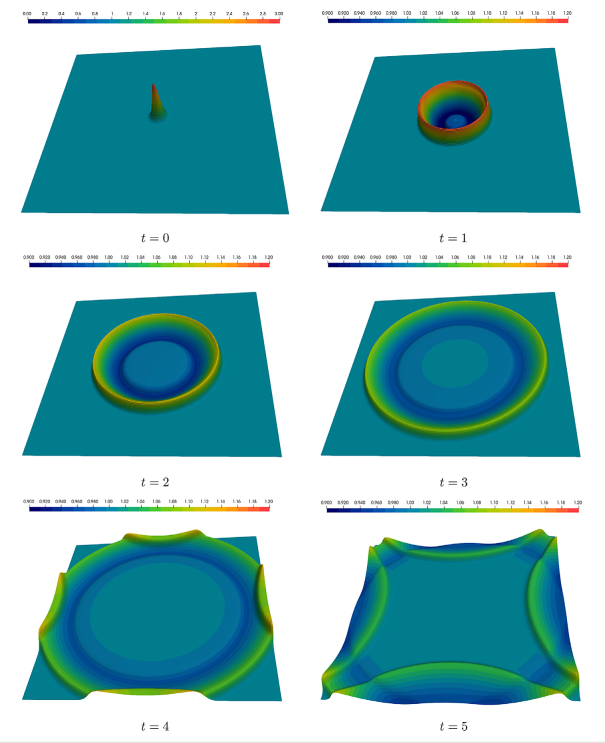
\includegraphics[width=\columnwidth]{fig1.png} % заглушка
\caption{Плотность в различные моменты времени.}
\label{fig:density_evolution}
\end{figure}

\begin{figure}[H]
\centering
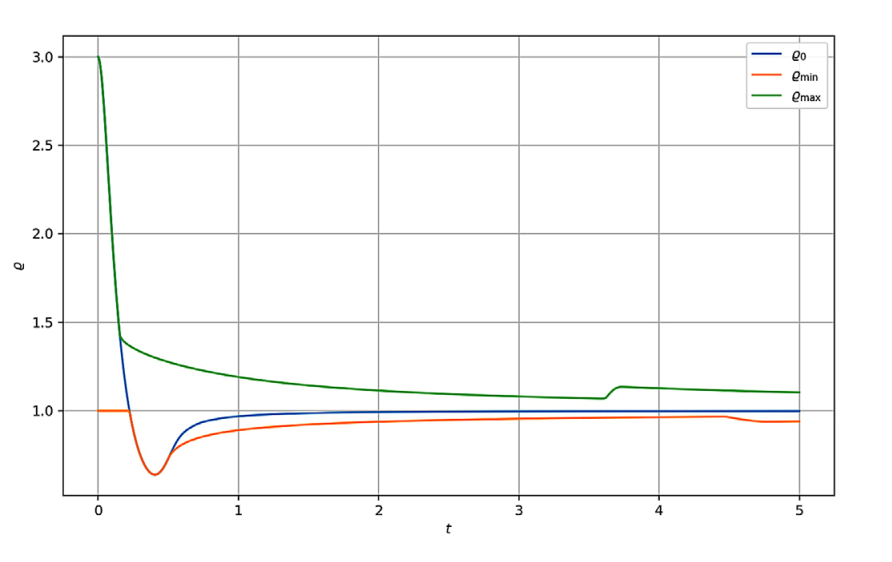
\includegraphics[width=\columnwidth]{fig2.png} % заглушка
\caption{Зависимости от времени плотности (центральное, максимальное и минимальное значения).}
\label{fig:density_time}
\end{figure}

\begin{figure}[H]
\centering
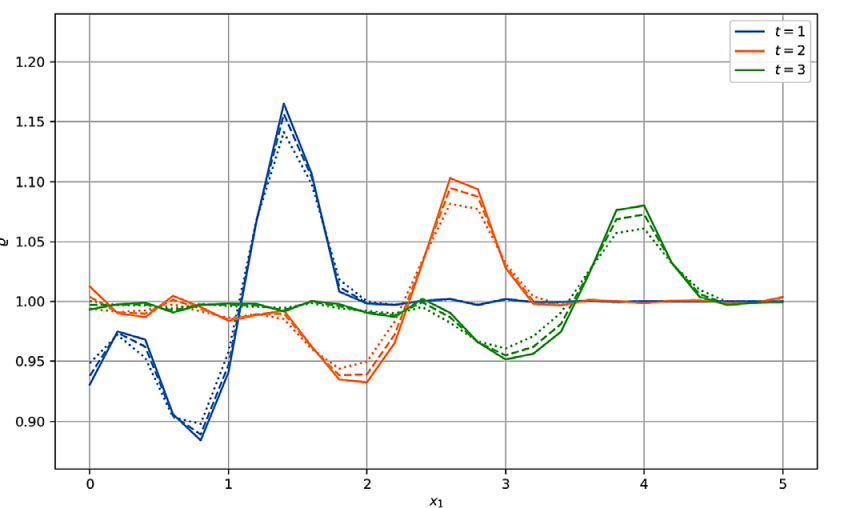
\includegraphics[width=\columnwidth]{fig3.png} % заглушка
\caption{Решение задачи в различные моменты времени, вычисленное на сетке \(M = 50\): пунктирная линия \(- \tau = 0.01\), штриховая \(- \tau = 0.005\), сплошная \(- \tau = 0.0025\).}
\label{fig:sol_M50}
\end{figure}

\begin{figure}[H]
\centering
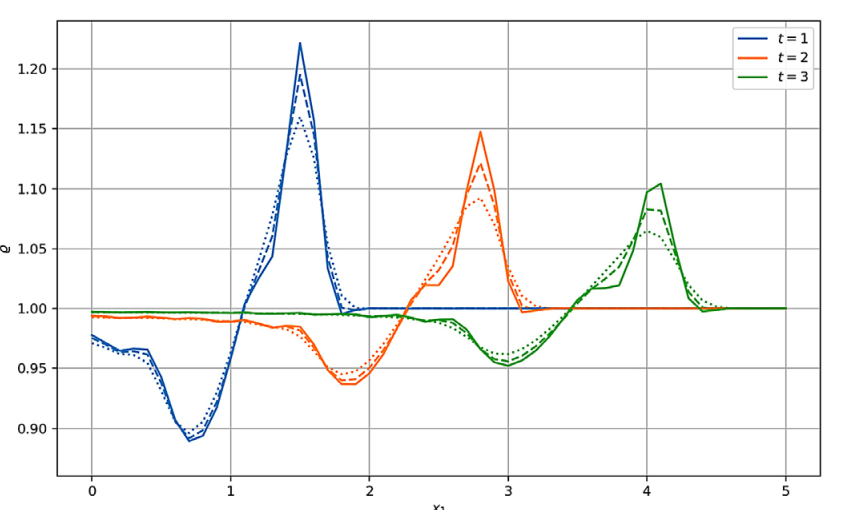
\includegraphics[width=\columnwidth]{fig4.png} % заглушка
\caption{Решение задачи в различные моменты времени, вычисленное на сетке \(M = 100\): пунктирная линия \(- \tau = 0.01\), штриховая \(- \tau = 0.005\), сплошная \(- \tau = 0.0025\).}
\label{fig:sol_M100}
\end{figure}

\begin{figure}[H]
\centering
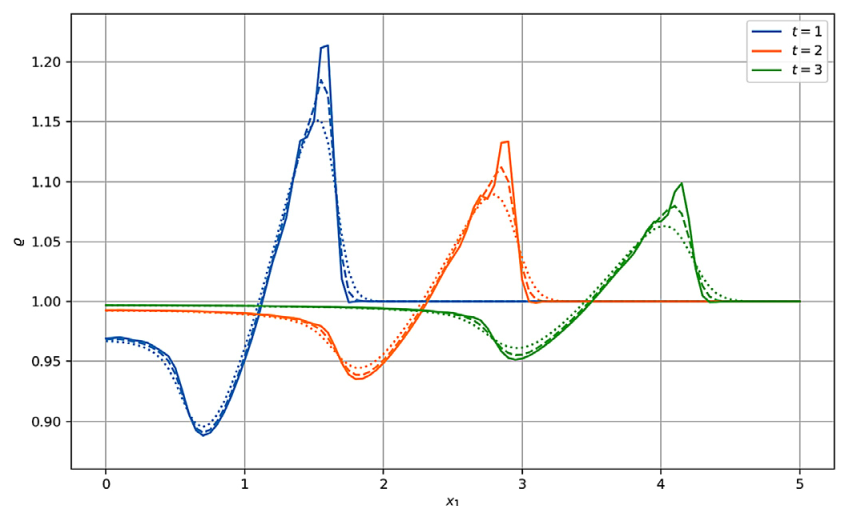
\includegraphics[width=\columnwidth]{fig5.png} % заглушка
\caption{Решение задачи в различные моменты времени, вычисленное на сетке \(M = 200\): пунктирная линия \(- \tau = 0.01\), штриховая \(- \tau = 0.005\), сплошная \(- \tau = 0.0025\).}
\label{fig:sol_M200}
\end{figure}

\begin{figure}[H]
\centering
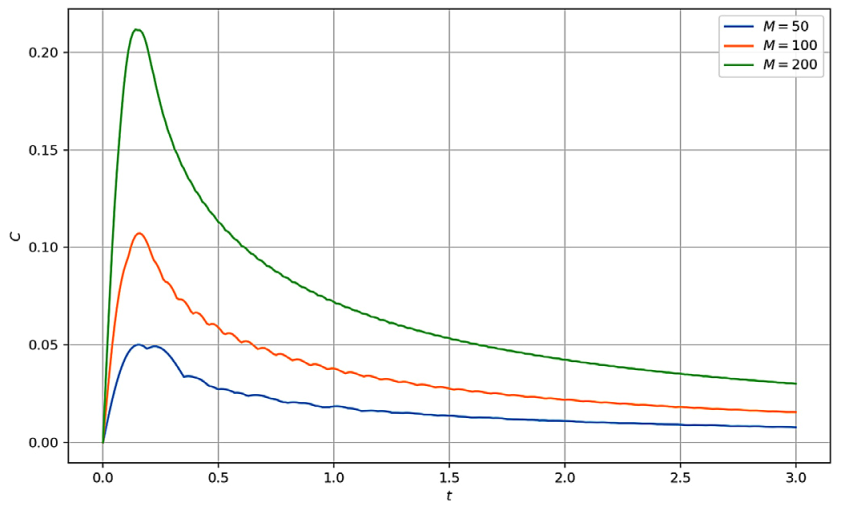
\includegraphics[width=\columnwidth]{fig6.png} % заглушка
\caption{Временная эволюция числа Куранта, вычисленного с \(\tau = 0.01\).}
\label{fig:courant}
\end{figure}


\subsection{Схема расщепления}

При использовании схемы расщепления (35)–(38) наибольший интерес представляет скорость сходимости итерационного процесса. Шаг по времени в расчетах был равен \(\tau = 0.005\). Мы представляем численные результаты для рассматриваемой модельной задачи, полученные на разных сетках по пространству. Зависимость решения от числа итераций для сетки с \(M = 50\) показана на рис. 7. На рис. 8 и 9 представлены аналогичные данные для сеток с \(M = 100\) и \(M = 200\) соответственно. Легко заметить, что на самой мелкой сетке (см. рис. 9) линеаризованная схема (33)–(34) \((K = 1\) в (35)–(38)) дает существенно немонотонное решение, которое монотонизируется на последующих итерациях.

\begin{figure}[H]
\centering
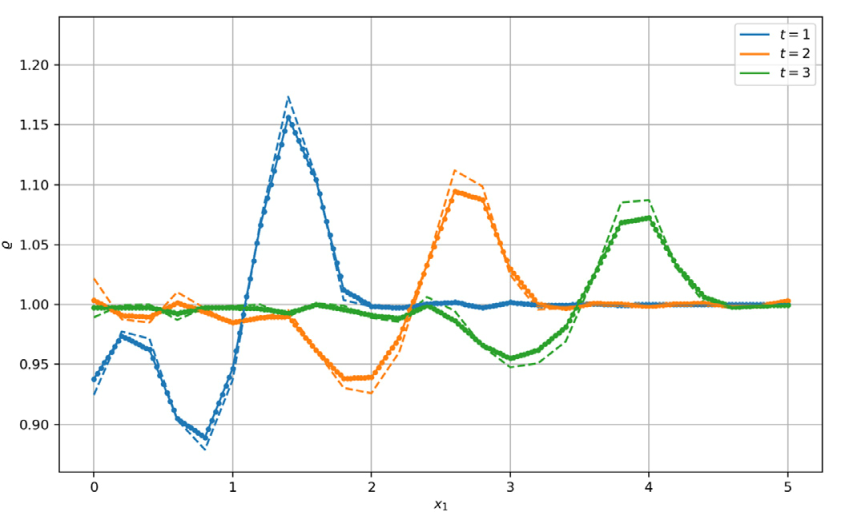
\includegraphics[width=\columnwidth]{fig7.png} % заглушка
\caption{Решение задачи в различные моменты времени, вычисленное на сетке \(M = 50\): штриховая линия \(-K = 1\), пунктирная \(-K = 2\), сплошная \(-K = 5\).}
\label{fig:iter_M50}
\end{figure}

\begin{figure}[H]
\centering
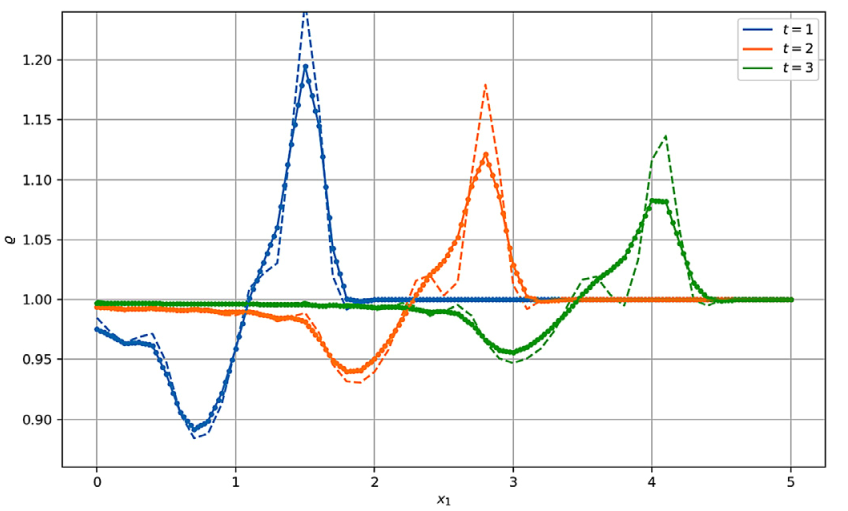
\includegraphics[width=\columnwidth]{fig8.png}
\caption{Решение задачи в различные моменты времени, вычисленное на сетке \(M = 100\): штриховая линия \(-K = 1\), пунктирная \(-K = 2\), сплошная \(-K = 5\).}
\label{fig:iter_M100}
\end{figure}

\begin{figure}[H]
\centering
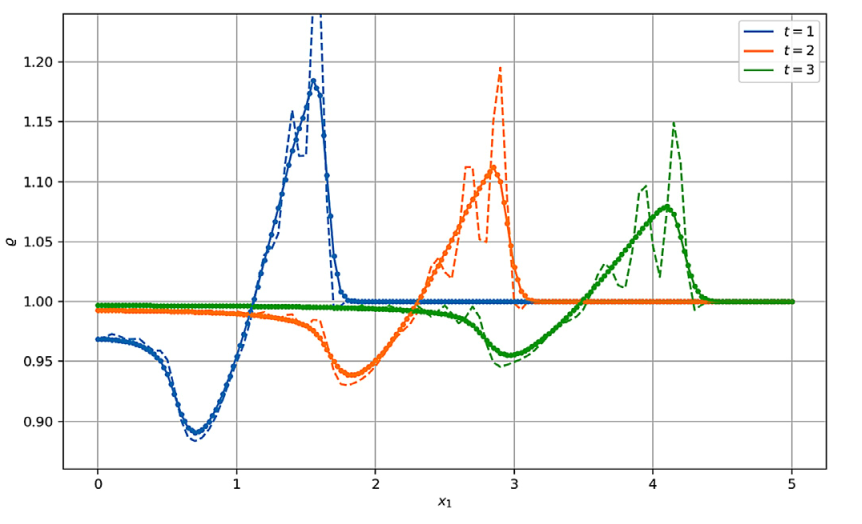
\includegraphics[width=\columnwidth]{fig9.png}
\caption{Решение задачи в различные моменты времени, вычисленное на сетке \(M = 200\): штриховая линия \(-K = 1\), пунктирная \(-K = 2\), сплошная \(-K = 5\).}
\label{fig:iter_M200}
\end{figure}

Основной вывод нашего исследования — демонстрация высокой вычислительной эффективности итерационной схемы расщепления (35)–(38). А именно, для рассматриваемых задач достаточно выполнить только две итерации с использованием (35)–(38).

Для вышеупомянутых методов шага по времени ключевым моментом является нарушение закона сохранения полной энергии. Для полностью неявной схемы (22)–(23) вместо сохранения энергии (см. оценку (32)) наблюдается убывание полной энергии.

Динамика полной механической энергии при использовании линеаризованной схемы (33)–(34) \((K = 1\) ) и итерационных схем расщепления (35)–(38)) для \(K = 5\) на различных сетках показана на рис. 10–12. Здесь, согласно (12), \(E(t_n)\) вычисляется в каждый момент времени следующим образом:

\begin{figure}[H]
\centering
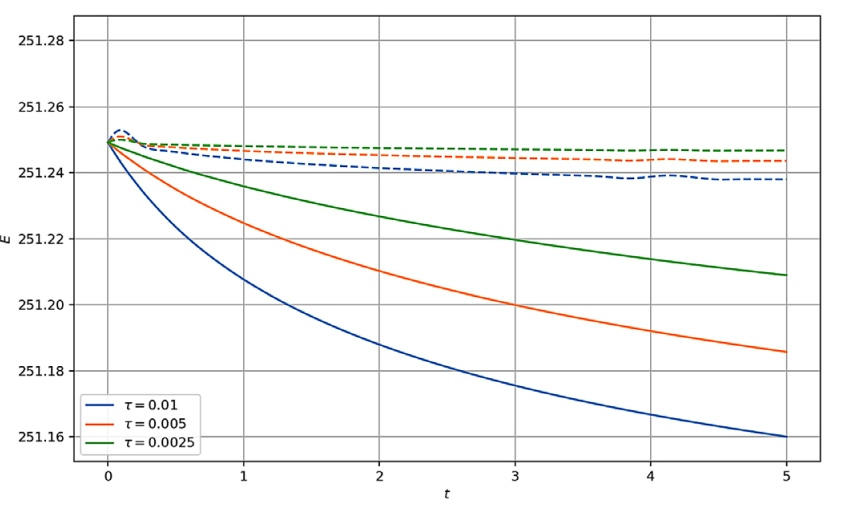
\includegraphics[width=\columnwidth]{fig10.png}
\caption{Временная эволюция полной механической энергии для различных шагов по времени, полученная на сетке с \(M = 50\): штриховая линия \(-K = 1\), сплошная \(-K = 5\).}
\label{fig:energy_M50}
\end{figure}

\begin{figure}[H]
\centering
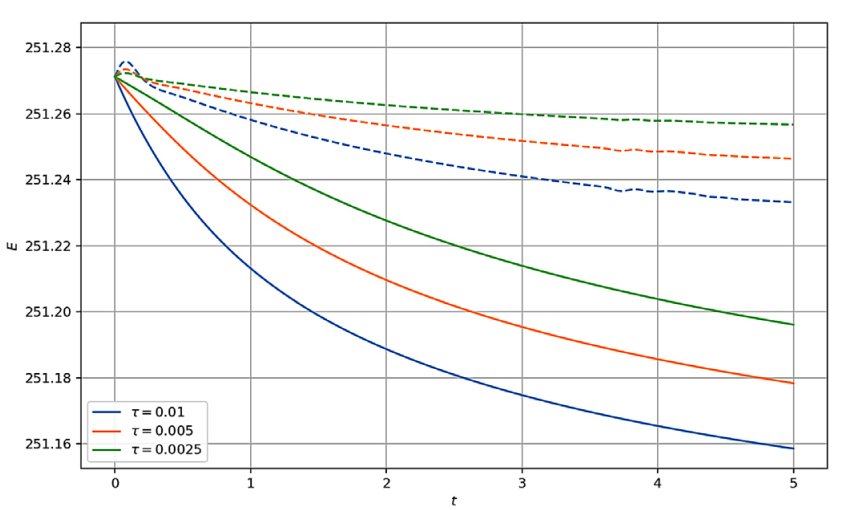
\includegraphics[width=\columnwidth]{fig11.png}
\caption{Временная эволюция полной механической энергии для различных шагов по времени, полученная на сетке с \(M = 100\): штриховая линия \(-K = 1\), сплошная \(-K = 5\).}
\label{fig:energy_M100}
\end{figure}

\begin{figure}[H]
\centering
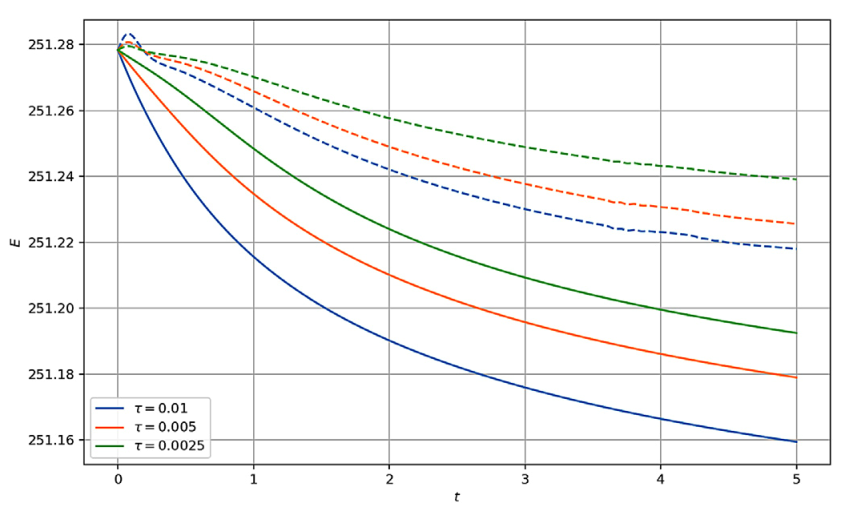
\includegraphics[width=\columnwidth]{fig12.png}
\caption{Временная эволюция полной механической энергии для различных шагов по времени, полученная на сетке с \(M = 200\): штриховая линия \(-K = 1\), сплошная \(-K = 5\).}
\label{fig:energy_M200}
\end{figure}

\[
E(t_n) = \int_{\Omega}\left(\frac{1}{2}\rho_n|\mathbf{u}_n|^2 + \Pi(\rho_n)\right)d\mathbf{x},\quad n = 0,1,\ldots ,N.
\]

Для \(K = 5\) энергия решения, полученного с помощью схемы расщепления (35)–(38), практически совпадает с энергией решения полностью неявной схемы (22)–(23). Это указывает на то, что закон сохранения полной энергии выполняется с хорошей точностью. Уменьшение шага по времени приводит к повышению точности выполнения закона сохранения.

\section{Заключение}

Для прогнозирования течений идеальной баротропной жидкости используется стандартная конечно-элементная аппроксимация по пространству вместе с полностью неявной двухслойной дискретизацией по времени (обратная схема Эйлера). Приближенное решение нелинейной задачи на новом временном уровне вычисляется с использованием итерационного метода Ньютона. Исследованы особенности сохранения массы, импульса и полной механической энергии. Предложена итерационная схема расщепления для динамических задач механики баротропной жидкости, в которой приближенное решение на новом временном уровне получается путем решения линейных задач для плотности и скорости. Эффективность полностью неявной схемы в подавлении нефизичных осцилляций продемонстрирована расчетами для модельной двумерной задачи. Такая монотонизация приближенного решения может быть скомбинирована с другими известными подходами. В частности, имеются хорошие перспективы для использования различных вариантов линейных и нелинейных аппроксимаций более высокого порядка по пространству.

\end{document}